\subsection{Introduction}
\subsubsection{What are names?}
Names are used to refer entities and these entities are usually accessed through an \emph{access point}, that is a special entity characterized by an address.
\textbf{Note that:}
\begin{itemize}
    \item An address is just a special case of name
    \item An entity can be accessed by several access points at the same time
    \item An entity can change its access points during its lifetime
\end{itemize}
So, it's better to use \emph{location-independent} names.\\
A name can be:
\begin{itemize}
    \item \textit{Global vs.local}
    \item \textit{Human-friendly vs. machine-friendly}
\end{itemize}

\subsubsection{Identifiers}
Resolving a name directly into an address does not work with mobility. For this reason we introduce identifiers, which are names they never change (during the entity lifetime). Moreover, each entity has exactly one identifier and this one is never assigned to another entity.\\
It's important to notice that using identifiers enables to split the problem of mapping a name to an entity and the problem of location the entity.
\subparagraph{Name resolution:} it's the process of obtaining the address of a valid access point of an entity having its name

\begin{center}\rule{3in}{0.4pt}\end{center}

\subsection{Naming schema}

There are three main naming schemas:
\begin{itemize}
    \item \emph{Flat naming}
    \item \emph{Structured naming}
    \item \emph{Attribute-based naming}
\end{itemize}

\subsubsection{Flat naming}
Names are flat, so they haven't any kind of structure. In practice, they're simple strings.\\
There are several name resolution processes:
\begin{itemize}
    \item \textit{Simple solutions}: they're based on broadcast or multicast approach or
      through pointers forwarding
    \item \textit{Home-based approaches}
    \item \textit{DHT}
    \item \textit{Hierarchical approaches}
\end{itemize}

\paragraph{Simple solutions}

They're designed for small-scale environments. There are three main ways to perform a simple resolution:

\begin{itemize}
    \item
        \textbf{Broadcast}: send \emph{find} message on broadcast channel and only the interested host replies. Obviously, since each host have to process the \emph{find} message there is a traffic and computational overhead
    \item 
        \textbf{Multicast}: same as broadcast, but send to multicast address to reduce the search scope
    \item
        \textbf{Forwarding pointers}: the idea is leave reference to the next location at the previous location. The main problem is that chains can became very long and broken links are fatal and, in general, there is a network latency increase. In order to reduce chain length, it can be adopted an adjusting procedure when searching an host, simply generate shortcuts to an host in order to reduce hops
\end{itemize}

\paragraph{Home-based approach}\label{home-based-approach}

The main idea is that one home node knows the location of the mobile
unit we're looking for. In fact, this approach is used mainly in Mobile
IP and 2.5G cellphone networks.

In order to work right, the home is assumed to be stable and it can be
replicated for robustness and the original IP of the host is effectively
used as an identifier.

There are also some problems. In particular, latency can increase of
there are too many steps towards the home. Moreover, the home address
has to be supported as long as the entity lives and since this address
is fixed, there may be an unnecessary burden when the entity permanently
moves to another location. In the end, there also a poor geographical
scalability problem, since entity can be next to client.

\paragraph{DHT}\label{dht}

The idea is to have an hash table distributed over several nodes,
organized and structured in an overlay network.

An example of DHT is \emph{Chord}:
\begin{figure}[h]
    \caption{Chord}
    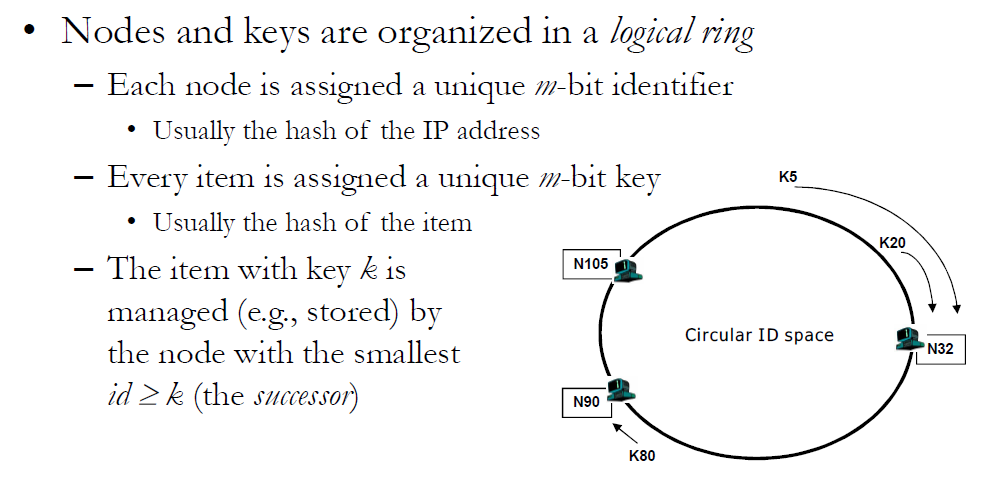
\includegraphics[width=\textwidth]{src/images/naming/dht.png}
    \centering
\end{figure}

The main idea is to jump as far as possible in order to be closer to the
possible solution. In order to do that, every node run very simple
operations, because the hash tables are small.

\paragraph{Hierarchical approach}

The idea is to have a tree, possibly balanced, and make a search that
first look in local registry to see if the entity is around and then, if
nothing has been found, contact the home.

The network is divided into domains, and the root domain spans the
entire network, while leaf nodes are typically a LAN or a cell. Thus,
all the nodes in the up of the tree have an huge router table. For this
reason, this solution can scale but not so good.

If it happens often that the search remains in the called node, it will
be efficient, otherwise we can have performance problems. We can cache
the information so the next time we have the same request, we can reply
in less time than before, though caching addresses directly is generally
inefficient.

In the hierarchical approach the updates start with insert request from
new location. Location records are created top down or bottom up, and
this one allows immediate queries.

\subsubsection{Structured naming}

In a structured naming system names are organized in namespaces, so we
have to introduce the concept of \emph{namespaces} which are labelled
graphs composed of leaf nodes, representing a name entity, and directory
nodes. In this case resources are referred through \emph{path names},
which can be \emph{relatives} or \emph{absolutes}.

Name spaces for a large scale, possibly worldwide, distributed\\system
are often distributed among different name servers, usually\\organized
hierarchically (DNS).

The name space is partitioned into layers:

\begin{itemize}
    \item \emph{Global level}
    \item \emph{Administration level}
    \item \emph{Managerial level}
\end{itemize}

Each node of the name space is assigned to a name server, so each name
server has a portion of name space.

There are also different needs in terms of performance between the
various levels. For example, I can accept that a name at the global
level is resolved in 2 seconds because it's stable stable and I can
cache it, but the same thing does not hold fit the managerial layer,
that has frequently edits and adds, so I cannot adopt cache policies.

\paragraph{Name resolutions approaches}

\begin{itemize}
    \item
        \textit{Iterative}: the client manages every single request to every single
        node
    \item
        \textit{Recursive}: the name servers manages the request to sub-servers. In
          this way, every layer must wait the under layer, so there are
          suspended threads, but we can apply some cache policies and so share
          the cache of different user requests
\end{itemize}

\paragraph{DNS}

Clients can request the resolution mode, but servers are not obliged to
comply. For the name resolution approach, a mixture of the two is used,
though global name servers typically support only iterative resolution.

In order to improve performance, caching and replication are massively
used, with up-to-date procedure and TTL attribute associated to
information which are useful to keep data consistent. However, transient
inconsistencies are allowed.

It's important to notice that mobile entities breaks the DNS
assumptions, i.e.~that the global/administration levels are quite
stables and the managerial levels are not. That's why phone numbers are
not managed in this way.

\subparagraph{What if a host is allowed to move?}

\begin{itemize}
\item
  If it stays in the original domain, so for example from
  \emph{ftp.example.com} to \emph{example.com}, there is no problem. The
  only thing to do is update the database of the domain server.
\item
  If a host moves to an entirely different domain, there are two main
  ways:
  \begin{itemize}
    \item
      Provide an IP address of the new location: lookups are ok, but further
      updates no longer \textit{localized}
    \item
      Provide the name of the new location: it will be necessary to perform
      two lookups and further updates no longer affected
  \end{itemize}
\end{itemize}

\subsubsection{Attribute-based naming}

The idea is to refer to entities not with their name but with a set of
attributes. In practice, each entity has a set of associated attribute.

They are usually implemented by using \emph{DBMS technology} and
Attribute based naming systems are usually called \emph{directory
services}.

\paragraph{LDAP}
\textit{LDAP} stands for Lightweight Directory Access Protocol

A typical approach to implement distributed directory services is to
combine structured with attribute-based naming.

An LDAP directory consist of a number of records, each is made as a
collection of \emph{} pairs and each attribute has a type. The
collection of all records in a \emph{LDAP} is called \emph{Directory
Information Base - DIB}.

\begin{figure}[h]
    \caption{Attribute naming example}
    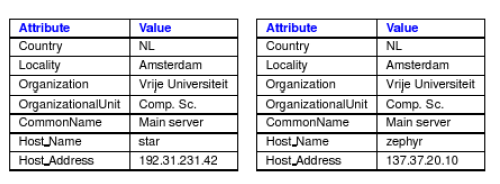
\includegraphics[width=\textwidth]{src/images/naming/attribute-naming.png}
    \centering
\end{figure}

This approach leads to build a \emph{directory information tree}, where
we use typically the mandatory attributes.
Each server is known as \emph{Directory Service Agent - DSA} and each client is known as \emph{Directory User Agent - DUA.}

In general, several DSA have to be accessed to resolve a query.

\begin{center}\rule{3in}{0.4pt}\end{center}

\subsection{Removing unreferenced entities}

It's important to remove unreferenced entities, mostly in some
distributed object platforms, like \textit{RMI}. The common used system is an
automatic garbage collector.

\subsubsection{Reference counting}

The idea of reference counting is to keep track of how many other
objects have been given references. Obviously, reliability must be
ensured, so exactly-once message delivery, but, since passing a
reference required three messages, there will be potential performance
issue in large-scale systems.

\subsubsection{Weighted reference counting}\label{weighted-reference-counting}

In order to avoid the communication problems, we can use only counter
decrements. The main idea is to have a counter that get lower and lower
as you pass a reference to an host. In practice, the counter tells us
how many reference are distributed in the network. If the total and
partial weights are equal the object can be removed, since it doesn't
have any other reference.

\begin{figure}[h]
    \caption{An example of reference counting}
    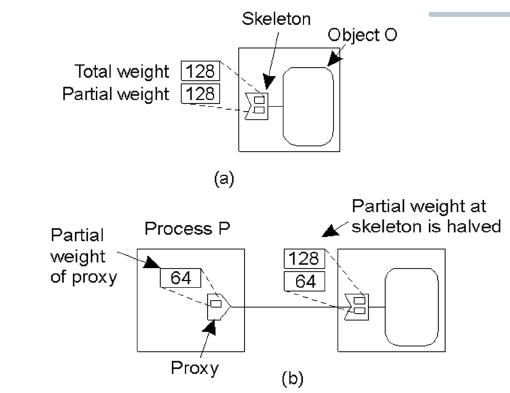
\includegraphics[scale=0.5]{src/images/naming/reference-counting.png}
    \centering
\end{figure}

This method has a limitation: we cannot generate more reference than
ones permitted by the total counters. In order to bypass this
limitation, we can introduce an additional hop to access the target
object.

\begin{figure}[h]
    \caption{Reference counting in case of counter equal to 1}
    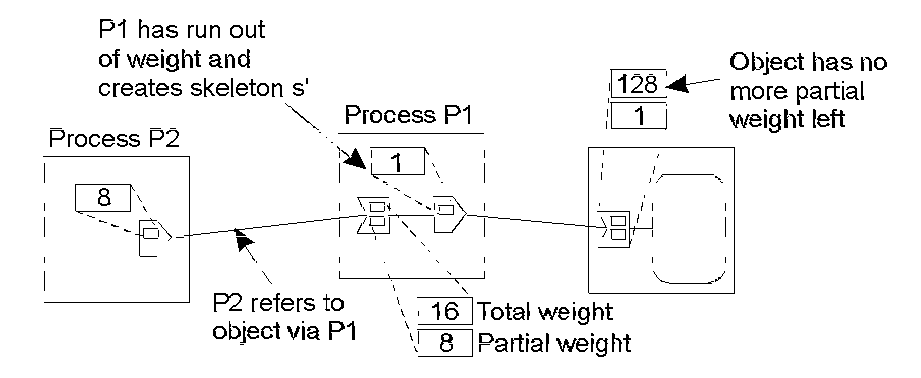
\includegraphics[scale=0.3]{src/images/naming/reference-counting-new-counter.png}
    \centering
\end{figure}

\subsubsection{Reference listing}

The problem of the mechanisms presented above is that they don't solve the
unreachability problems. The idea to solve this problem is, instead of keeping track of the number of references, keep
track of the identities of the proxies.\\
With this method we have several advantages:
\begin{itemize}
    \item Insertion and deletion of references must still be acknowledged, so we can send many messages with the same effect
    \begin{itemize}
        \item Related to the point before, non-reliable communication can be used
    \end{itemize}
    \item It's easy to maintain the list consistent w.r.t. network failures,
      applying some policies (\emph{e.g.~ping})
\end{itemize}

\textbf{Note that:} this method is used by \emph{Java RMI}

\subsubsection{Identifying unreachable entities}

\emph{Mark-and-sweep} on uniprocessor systems:
\begin{enumerate}
    \item
      Marks accessible entities by following references
      
    \item
      Initially all nodes white
    \begin{itemize}
        \item A node is coloured grey when reachable from a root but some of its
          references still need to be evaluated
        \item A node is coloured black after it turned grey and all its outgoing
          references have been marked grey
    \end{itemize}
    
    \item
      Second phase exhaustively examines memory to locate entities not
      marked and removes them
      \begin{itemize}
        \item Garbage collects all white nodes
      \end{itemize}
\end{enumerate}

There is also a distributed version of this algorithm, in which garbage
collectors run on each site.
